\chapter{Network Framework}\label{ch:Network Framework}

Completing the second part of the project requires implementing the Speech Recogniser in a distributed manner. High level, the system requires open access over a network, local or otherwise. Low level, the recogniser must be able to communicate over the available network. In order to demonstrate the system's complete functionality, a Virtual Private Network (VPN) is used to provide open access between devices and sockets are used to send data through the network.

\section{Virtual Private Network (VPN)}

The VPN extends a private network over a public network and enables devices to send and receive data across shared or public networks, in the same way as if they would be directly connected to the same network. 
Due to the fact that multiple devices are in various locations and on different networks, some of which have security protocols enabled, direct communication between these devices is not possible without a VPN.\\\\
OpenVPN is the open-source software application that was utilized here. 
It implements VPN techniques for creating secure point-to-point connections in routed or bridged configurations and remote access. 
A custom security protocol, based on SSL/TLS is enforced on the network, and it is capable of traversing network address translators (NATs) and firewalls.\\
For the current project, OpenVPN was used in a multiclient-server configuration. Authentication certificates were released for every client that required access on the network.

\begin{figure}[h]
	\centering
	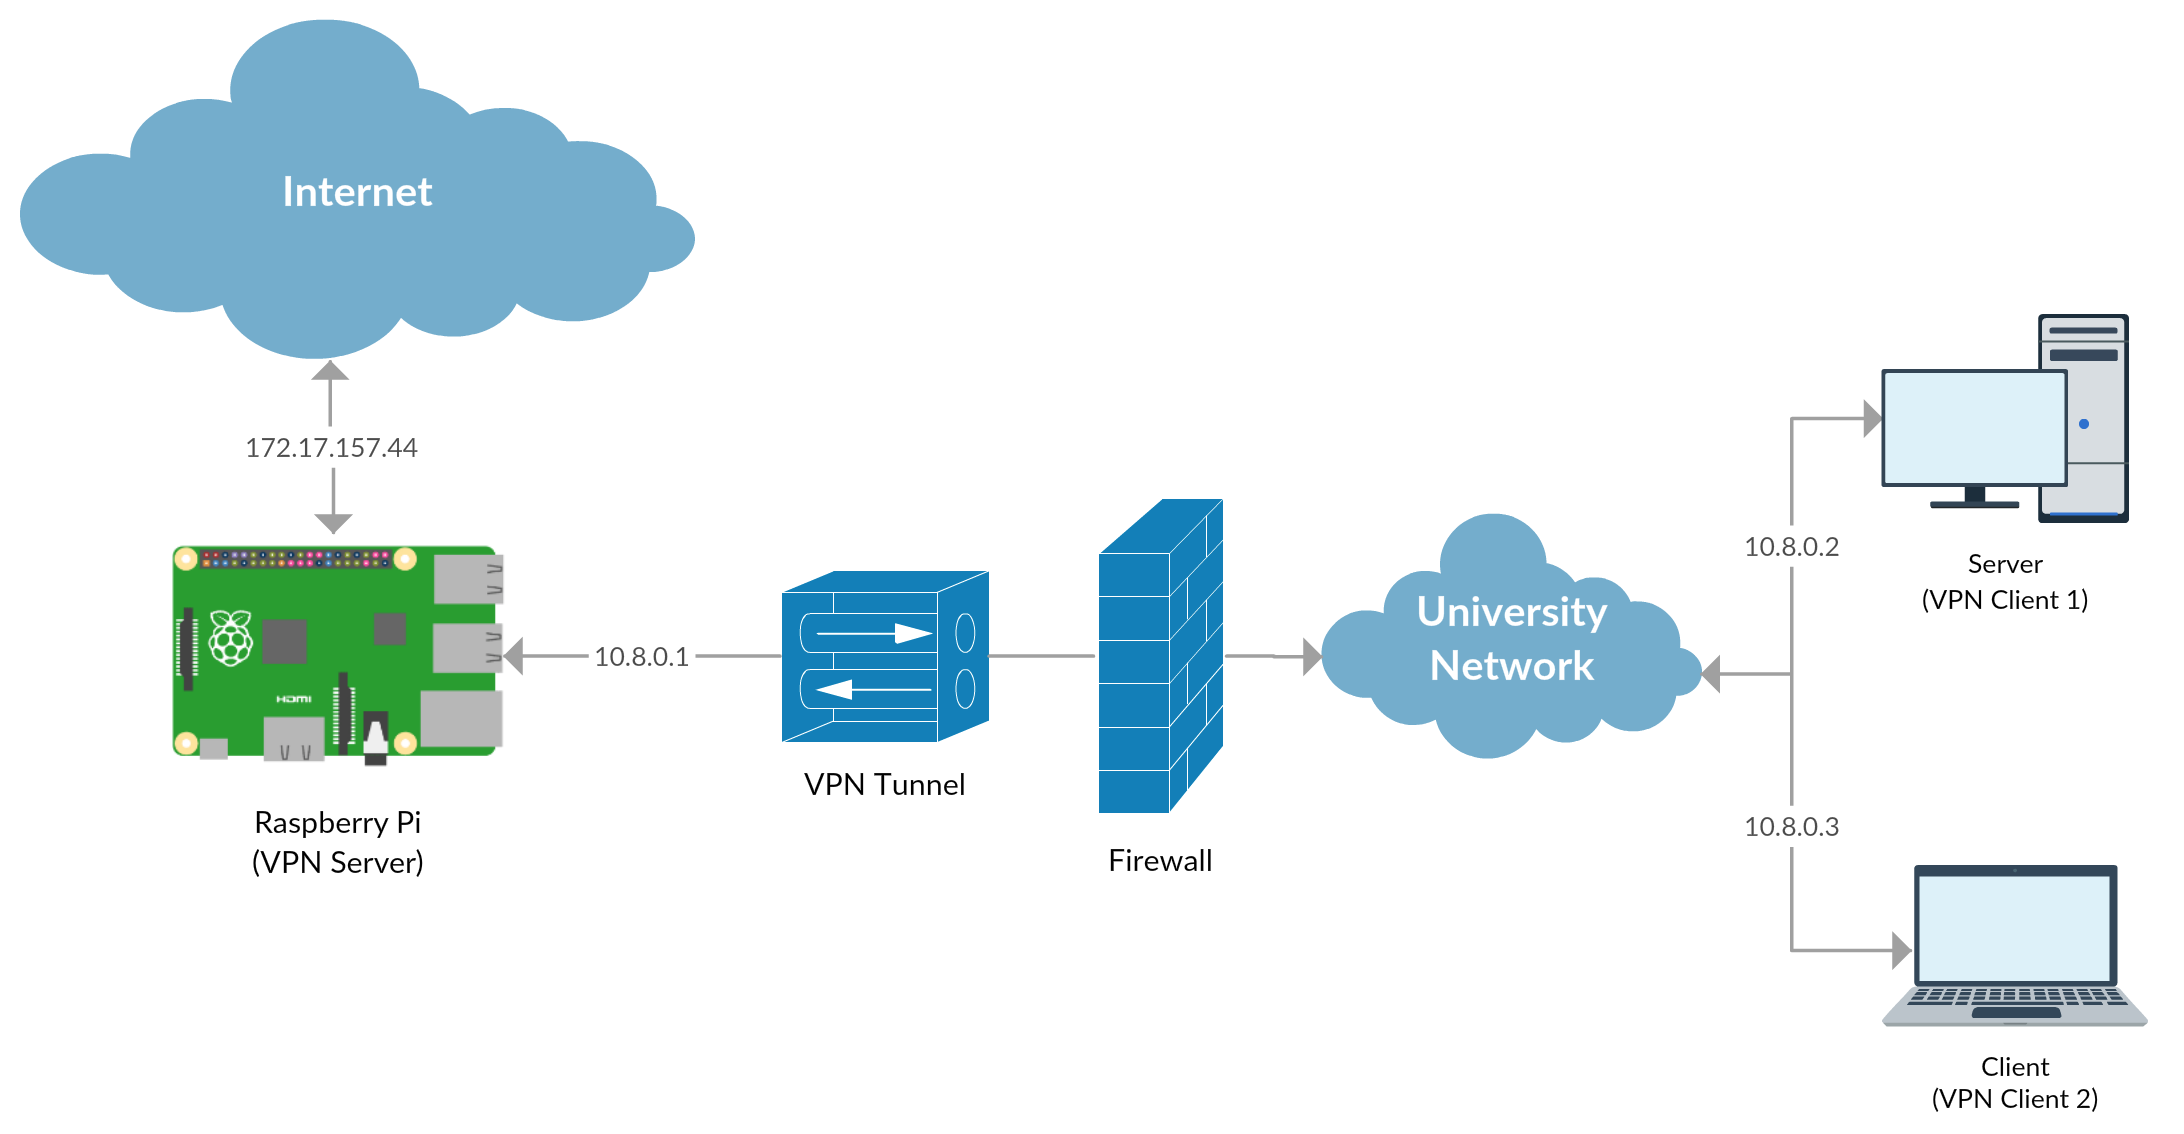
\includegraphics[width=\textwidth]		
	{network_framework/client_server_framework}
	\caption{Virtual private network to university.}
	\label{fig:vpn_uni_diagram}
\end{figure}

\section{Sockets}